\documentclass[journal=jacsat,manuscript=article]{achemso}
\usepackage[version=3]{mhchem}
\usepackage[english]{babel}
\usepackage[utf8]{inputenc}
\usepackage{anysize}
\usepackage{float}
\usepackage{graphicx}


% AUTHORS
\author{Cristina Ruiz}
\altaffiliation{Both authors have equally contributed}
\author{Álvaro Raya-Barón}
\altaffiliation{Both authors have equally contributed}
\author{Manuel A. Ortuño}
\affiliation[b]{Institute of Chemical Research of Catalonia (ICIQ), The Barcelona Institute of Science and Technology (BIST), Av. Països Catalans 16, 43007 Tarragona, Spain.}
\email{mortuno@iciq.es}
\author{Ignacio Fernández}
\email{ifernan@ual.es}
\affiliation[a]{Department of Chemistry and Physics, Research centre CIAIMBITAL, Ctra. Sacramento, s/n, 04120 Almería, Spain.}

%FALTAN LAS ABREVIATURAS Y PALABRAS CLAVE

% TITLE
\title{Accelerating role of deaggregation agents in lithium-catalysed hydrosilylation of carbonyl compounds} %Electronic supplementary information (ESI) available: Kinetic plots, NMR spectra, computational details, intermediate and transition state structures. See DOI: 10.1039/d0dt01540g

% MANUSCRIPT
\begin{document}
\maketitle

	% ABSTRACT
	
	\begin{abstract}
		% https://github.com/cristiruizblaze/proyecto_final{\tiny }
		
		A combined computational and experimental approach demonstrates the accelerating role of deaggregation agents, especially HMPA, in the Li-catalysed hydrosilylation of acetophenone in THF solution under very mild conditions.
	\end{abstract}
	
	% INTRODUCTION
	
	\section{Introduction}
	The reduction of carbonyl groups into alcohols is of wide interest in synthetic chemistry and therefore, constant efforts are	put into developing new efficient methodologies and perfecting the existing ones. Catalytic hydrosilylation1 has emerged as a convenient method as it operates under mild conditions and	combines an exceptional reducing capability with a high selectivity that can be finely tuned via catalyst design.
	
	% STATE OF THE ART
	
	\section{State of the art}
	Many Earth-abundant first-row transition metals, specially iron,2,3 have been tested in catalytic hydrosilylation of carbonyl compounds, as they are usually more environmentally-friendly and less toxic than their second- and third-row counterparts. Alkali metal salts have also been explored as alternative catalysts, initially by the groups of Corriu4 and Hosomi,5 and later by Beller6 and Nikonov,7 among others. Such compounds have been employed to promote hydrosilylation due to their basic character via formation of a pentacoordinated hydridosilicate,6–8 usually neglecting any relevant role of the alkali cation in the reaction mechanism. We recently reported	the hydrosilylation of carbonyl compounds catalysed by lithiated hydrazones.9 However, full understanding at atomic level of detail is still needed for the rational design of catalysts and reaction conditions.
	\\Herein we join computational and experimental efforts to understand and optimise processes catalysed by alkali–metal amides.10 Following theoretical guidance, we demonstrate how deaggregation agents (DAs) can efficiently accelerate hydrosilylation of carbonyl compounds in the presence of readily available lithium amides (Scheme 1) under very mild conditions such as room temperature and very low catalyst loading.
	\\
	
	\begin{figure}[h]
	\includegraphics[width=0.6\textwidth]{figures/Síntesis.PNG}
	\centering
	\caption{Hydrosilylation of ketones catalysed by the combination of	Li-amides with deaggregation agents}
	\centering
	\label{Scheme1}
	\end{figure}	

	% RESULTS AND DISCUSSION
	
	\section{Results and discussion}
	First, we computed the reaction mechanism for acetophenone and (MeO)2MeSiH using lithium diisopropylamide (LDA) as catalyst.9 The proposed reaction mechanism entails an activation step (Scheme 2a) prior to the catalytic cycle (Scheme 2b). We start from the LDA dimer 1 in THF solution. Dissociation of 111 via coordination of carbonyl and silane reactants yields the monomeric intermediates 2 and 3 at 17.8 kcal mol-1. The Si-H bond is then activated via amide nucleophilic attack,12 giving rise to a putative Li–hydride 5 as in Fe analogues 13,14 via -25 kcal mol-1. Although such transient intermediate would be very difficult to detect experimentally, similar species have been proposed in related literature. 15,16 Insertion of acetophenone into the Li-H bond generates an alkoxide 6 which activates a silane molecule 8 through a pentacoordinated hydridosilicate. Subsequent	hydride transfer releases the product and regenerates the Li-H species 5. According to the reaction profile (Scheme 2c), all relative activation Gibbs energies within the cycle are rather small, in the range of 7-10 kcal mol-1, with an overall value of 9.5 kcal mol-1 above 6. The most energy-demanding steps concern the initial dissociation of 1 to monomer 3 via 17.8 kcal mol-1 followed by the formation of hydride 5 via 25.4 kcal mol-1.
	
	\begin{center}
	\begin{minipage}{0.6\textwidth} 
		\begin{figure}[H]
			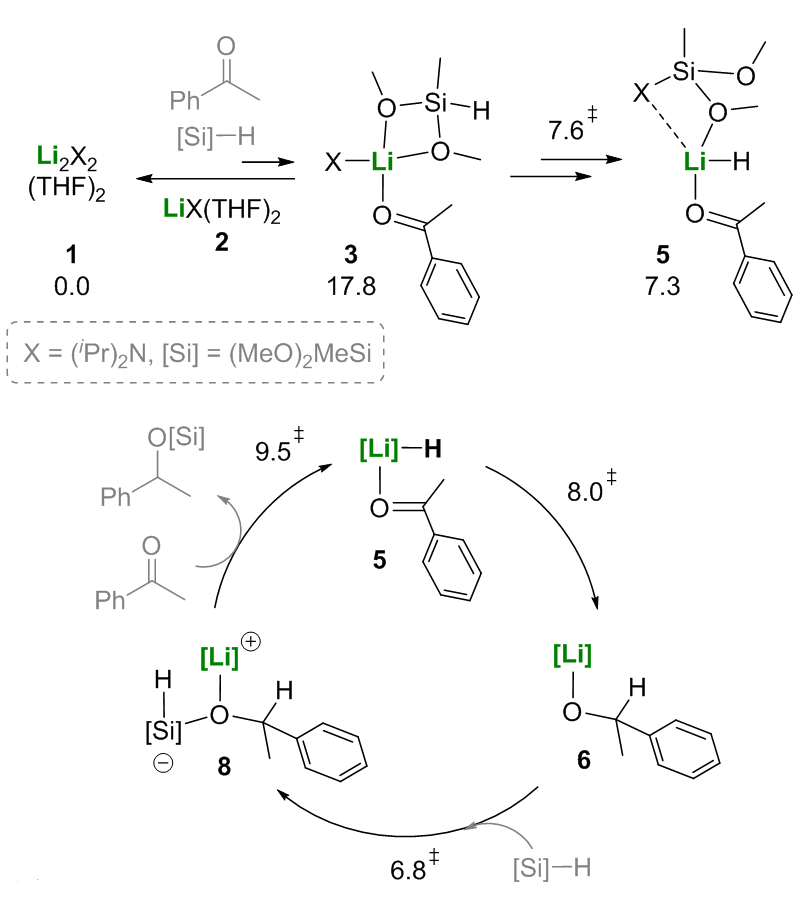
\includegraphics[width=\textwidth]{figures/Ciclo.PNG}
			\end{figure}
	\end{minipage}

	\begin{minipage}{0.6\textwidth} 
		\begin{figure}[H]
			\includegraphics[width=\textwidth]{figures/Energía.PNG}
			\caption{\label{Scheme2} Computed (a) pre-activation step and catalytic cycle, and (b) reaction profile for the hydride-mediated Li-catalysed hydrosilylation of acetophenone. All Gibbs energies are given in THF in kcal mol-1.}
		\end{figure}
	\end{minipage}
	\end{center}


\end{document}